%-------------------------------------------------------------------------------
%                                PREAMBLE
%-------------------------------------------------------------------------------
\documentclass[usenames,dvipsnames,svgnames,10pt,aspectratio=169]{beamer}
%
\usefonttheme{professionalfonts}
% This theme uses TIKZ: compile twice with PDFLaTeX or LuaLaTeX.
%
%  Options:
%  - [clean]:    clean slides, i.e. logos and footbar are removed
%  - [kth]:      footbar style inspierd to the official KTH template
%  - [nicewave]: a different style of wave is used (not approved by FLOW)
%
\usetheme[clean]{flow}

\usepackage{tikz}
\usetikzlibrary{arrows}
\usetikzlibrary{shapes.geometric, math, positioning, calc, patterns, angles, quotes}
\usetikzlibrary{patterns.meta,decorations.pathmorphing}

\newcommand{\semaphore}[3]{% #1: color of circle,
                           % #2: color of semicircle
                           % #3: angle of semicircle 
  \tikz[node distance=0mm,baseline]
       {
         \node (s1) [circle, fill=#1, minimum size=6mm] {};
         \node      [semicircle, fill=#2, 
           inner sep=0pt, outer sep=0pt, minimum size=3mm,
           anchor=south,
           at={(s1.center)}, rotate=#3] {};
       }
}

\usepackage[]{circuitikz}

\usepackage{pgfplots}
\usepgfplotslibrary{polar}

\usepackage{hyperref,graphicx,lmodern}
\usepackage[utf8]{inputenc}
\usepackage{media9}
\usepackage{xcolor}
\usepackage{stmaryrd}
\usepackage{nicefrac}
\usepackage{multimedia}
\usepackage{multicol}
\usepackage{upgreek}
\usepackage[]{bm}
\usepackage[]{url}
\usepackage[]{animate}
\usepackage{amsmath}

\graphicspath{{imgs/}}
\setbeamertemplate{blocks}[rounded][shadow=true]

\DeclareMathOperator*{\maximize}{maximize~}

%-------------------------------------------------------------------------------
%                                TITLE PAGE
%-------------------------------------------------------------------------------
\title[Nonlinear physics] % Short title used in footline
{
	Conservative, reversible and \\
  dissipative dynamical systems
}

\author[J.-Ch.~Loiseau] % Presenting author in short form used in footline
{
	\underline{Jean-Christophe Loiseau}
}
% - Give the names in the same order as the appear in the paper.
% - Underline the presenting author.

\institute[unused]
{
	\url{jean-christophe.loiseau@ensam.eu} \\
	Laboratoire DynFluid \\
	Arts et M\'etiers, France.
}
% Keep it simple, no one is interested in your street address.

% University logo(s)
\logot{\includegraphics[width=.128\paperwidth]{DynFluid_logo}}  % Top logo
\logob{\includegraphics[width=0.128\paperwidth]{ENSAM_logo}} % Bottom logo
% \logoc[{\includegraphics[width=.128\paperwidth]{limsi}}]{\includegraphics[width=.128\paperwidth]{limsi}} % Corner logo
%
% Cover image: \cvrimg{x position}{y position}{cover image}
\cvrimg{.77}{.8}{\includegraphics[width=.4\paperwidth]{cover.png}}

\date[unused]{Physique non-lin\'eaire -- 2019-2020}

\begin{document}

\titleframe	% Print the title as the first slide

%-------------------------------------------------------------------------------
%                           PRESENTATION SLIDES
%-------------------------------------------------------------------------------

\begin{frame}[t, c]{Two-dimensional systems}{Two major classes of dynamical systems}
  \begin{minipage}{.48\textwidth}
    \centering

    \textbf{Conservative}
    %
    \[
    \begin{aligned}
      \dot{x} & = y \\
      \dot{y} & = -\sin(x) \end{aligned}
    \]
  \end{minipage}%
  \hfill
  \begin{minipage}{.48\textwidth}
    \centering
    \textbf{Dissipative}
    %
    \[
    \begin{aligned} \dot{x} & = y \\
      \dot{y} & = -y - x - x^3
    \end{aligned}
    \]
  \end{minipage}

  \vspace{1cm}
\end{frame}

\begin{frame}[t, c]{Two-dimensional systems}{Conservative systems}
  \begin{minipage}{.68\textwidth}
    \begin{overprint}

      \onslide<1>
      The equations of motion of many physical systems can be derived from Newton's principles.
      They are of the form
      %
      \[
      m \ddot{x} = F(x)
      \]
      %
      where $F(x)$ is independent of both $\dot{x}$ and $t$, i.e. the system is autonomous and frictionless.

      \onslide<2>
      Under this assumption, we can show that $F(x)$ derives from a potential, i.e.
      %
      \[
      F(x) = -\dfrac{dV}{dx}
      \]
      %
      such as the gravitational potential energy $V(x) = mgx$ or the elastic potential energy of a spring $V(x) = \dfrac{1}{2} k x^2$.

    \end{overprint}
  \end{minipage}%
  \hfill
  \begin{minipage}{.28\textwidth}
    \centering
    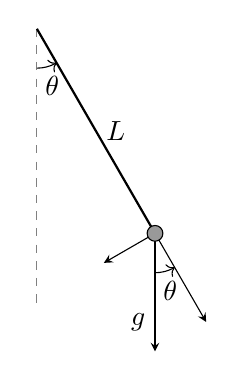
\begin{tikzpicture}
      % save length of g-vector and theta to macros
      \pgfmathsetmacro{\Gvec}{1.5}
      \pgfmathsetmacro{\myAngle}{30}
      % calculate lengths of vector components
      \pgfmathsetmacro{\Gcos}{\Gvec*cos(\myAngle)}
      \pgfmathsetmacro{\Gsin}{\Gvec*sin(\myAngle)}
      
      \coordinate (centro) at (0,0);
      \draw[dashed,gray,-] (centro) -- ++ (0,-3.5) node (mary) [black,below]{$ $};
      \draw[thick] (centro) -- ++(270+\myAngle:3) coordinate (bob) node[midway, right] {$L$};
      \pic [draw, ->, "$\theta$", angle eccentricity=1.5] {angle = mary--centro--bob};
      %\draw [blue,-stealth] (bob) -- ($(bob)!\Gcos cm!(centro)$);
      \draw [-stealth] (bob) -- ($(bob)!-\Gcos cm!(centro)$)
      coordinate (gcos)
      node[midway,above right] {};
      \draw [-stealth] (bob) -- ($(bob)!\Gsin cm!90:(centro)$)
      coordinate (gsin)
      node[midway,above left] {};
      \draw [-stealth] (bob) -- ++(0,-\Gvec)
      coordinate (g)
      node[near end,left] {$g$};
      \pic [draw, ->, "$\theta$", angle eccentricity=1.5] {angle = g--bob--gcos};
      \filldraw [fill=black!40,draw=black] (bob) circle[radius=0.1];
    \end{tikzpicture}
  \end{minipage}

  \vspace{1cm}
\end{frame}

\begin{frame}[t, c]{Two-dimensional systems}{Conservative systems}
  \begin{minipage}{.68\textwidth}
    From there, the equations of motion can be rewritten as
    %
    \[
    m \ddot{x} + \dfrac{dV}{dx}  = 0.
    \]
    %
    One can then show that
    %
    \[
    \dfrac{d}{dt} \left( \dfrac{1}{2} m \dot{x}^2 + V(x) \right) = 0.
    \]
    %
    The quantity $\dfrac{1}{2} m \dot{x}^2 + V(x)$ is thus \alert{\textbf{conserved}} over time.
    
  \end{minipage}%
  \hfill
  \begin{minipage}{.28\textwidth}
    \centering
    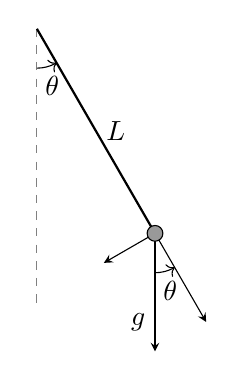
\begin{tikzpicture}
      % save length of g-vector and theta to macros
      \pgfmathsetmacro{\Gvec}{1.5}
      \pgfmathsetmacro{\myAngle}{30}
      % calculate lengths of vector components
      \pgfmathsetmacro{\Gcos}{\Gvec*cos(\myAngle)}
      \pgfmathsetmacro{\Gsin}{\Gvec*sin(\myAngle)}
      
      \coordinate (centro) at (0,0);
      \draw[dashed,gray,-] (centro) -- ++ (0,-3.5) node (mary) [black,below]{$ $};
      \draw[thick] (centro) -- ++(270+\myAngle:3) coordinate (bob) node[midway, right] {$L$};
      \pic [draw, ->, "$\theta$", angle eccentricity=1.5] {angle = mary--centro--bob};
      %\draw [blue,-stealth] (bob) -- ($(bob)!\Gcos cm!(centro)$);
      \draw [-stealth] (bob) -- ($(bob)!-\Gcos cm!(centro)$)
      coordinate (gcos)
      node[midway,above right] {};
      \draw [-stealth] (bob) -- ($(bob)!\Gsin cm!90:(centro)$)
      coordinate (gsin)
      node[midway,above left] {};
      \draw [-stealth] (bob) -- ++(0,-\Gvec)
      coordinate (g)
      node[near end,left] {$g$};
      \pic [draw, ->, "$\theta$", angle eccentricity=1.5] {angle = g--bob--gcos};
      \filldraw [fill=black!40,draw=black] (bob) circle[radius=0.1];
    \end{tikzpicture}
  \end{minipage}

  \vspace{1cm}
\end{frame}

\begin{frame}[t, c]{Two-dimensional systems}{Conservative systems}
  \begin{minipage}{.68\textwidth}
    For the pendulum, the equations of motions are
    %
    \[
    \underbrace{mL\ddot{\theta}}_{\text{Acceleration}} + \underbrace{mg \sin(\theta)}_{\text{-Weight}} = 0
    \]
    %
    Multiplying by the velocity $L \dot{\theta}$ yields
    %
    \[
    \dfrac{d}{dt} \left( \dfrac{1}{2} m(L\dot{\theta})^2 - mgL \cos(\theta) \right) = 0.
    \]
    %
    We thus recover that the \alert{\textbf{total energy}} of the system is conserved (in the absence of friction).
  \end{minipage}%
  \hfill
  \begin{minipage}{.28\textwidth}
    \centering
    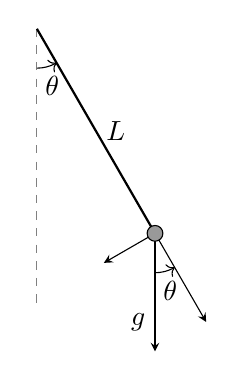
\begin{tikzpicture}
      % save length of g-vector and theta to macros
      \pgfmathsetmacro{\Gvec}{1.5}
      \pgfmathsetmacro{\myAngle}{30}
      % calculate lengths of vector components
      \pgfmathsetmacro{\Gcos}{\Gvec*cos(\myAngle)}
      \pgfmathsetmacro{\Gsin}{\Gvec*sin(\myAngle)}
      
      \coordinate (centro) at (0,0);
      \draw[dashed,gray,-] (centro) -- ++ (0,-3.5) node (mary) [black,below]{$ $};
      \draw[thick] (centro) -- ++(270+\myAngle:3) coordinate (bob) node[midway, right] {$L$};
      \pic [draw, ->, "$\theta$", angle eccentricity=1.5] {angle = mary--centro--bob};
      %\draw [blue,-stealth] (bob) -- ($(bob)!\Gcos cm!(centro)$);
      \draw [-stealth] (bob) -- ($(bob)!-\Gcos cm!(centro)$)
      coordinate (gcos)
      node[midway,above right] {};
      \draw [-stealth] (bob) -- ($(bob)!\Gsin cm!90:(centro)$)
      coordinate (gsin)
      node[midway,above left] {};
      \draw [-stealth] (bob) -- ++(0,-\Gvec)
      coordinate (g)
      node[near end,left] {$g$};
      \pic [draw, ->, "$\theta$", angle eccentricity=1.5] {angle = g--bob--gcos};
      \filldraw [fill=black!40,draw=black] (bob) circle[radius=0.1];
    \end{tikzpicture}
  \end{minipage}

  \vspace{1cm}
\end{frame}

\begin{frame}[t, c]{Two-dimensional systems}{Conservative systems}
  \begin{minipage}{.48\textwidth}
    For a conservative system, the energy remains constant along a given trajectory.

    \bigskip

    Fixed points cannot be attractive and the trajectories are closed orbits.
  \end{minipage}%
  \hfill
  \begin{minipage}{.48\textwidth}
    \centering
    \begin{tikzpicture}
      \draw[->, >=stealth] (-1.25*pi/2, 0) -- (1.25*pi/2, 0) node[below] {$\theta$};
      \draw[->, >=stealth] (0, -pi/2) -- (0, pi/2) node[left] {$\dot{\theta}$};

      \draw[->, >=stealth, gray, smooth, thick] plot file{traj1bis.txt};
      \draw[->, >=stealth, gray, smooth, thick] plot file{traj2bis.txt};
      \draw[->, >=stealth, gray, smooth, thick] plot file{traj3bis.txt};
      \draw[->, >=stealth, gray, smooth, thick] plot file{traj4bis.txt};
      \draw[->, >=stealth, gray, smooth, thick] plot file{traj5bis.txt};

      \node[circle, fill=black, draw=black, inner sep=0pt, minimum size=4pt] (a) at (0, 0) {};
      \node[circle, fill=white, draw=black, inner sep=0pt, minimum size=4pt] (a) at (pi/2, 0) {};
      \node[circle, fill=white, draw=black, inner sep=0pt, minimum size=4pt] (a) at (-pi/2, 0) {};

    \end{tikzpicture}
  \end{minipage}

  \vspace{1cm}
\end{frame}

\begin{frame}[t, c]{Conservative systems}{Hamiltonian formalism}
  \begin{minipage}{.68\textwidth}
    Conservative systems are crucially important in physics and gave rise to \alert{\textbf{Hamiltonian mechanics}} (in opposition to Lagrangian mechanics).

    \bigskip

    In a suitable reference frame $(\bm{p}, \bm{q})$ where $\bm{p}$ and $\bm{q}$ are the \alert{\textbf{generalized coordinates}}, the equations of motion take a special form known as the \alert{\textbf{Hamilton equations}}.
  \end{minipage}%
  \hfill
  \begin{minipage}{.28\textwidth}
    \centering
    \textbf{Hamilton equations}
    \[
    \begin{aligned}
      \dot{\bm{p}} & = -\dfrac{d\mathcal{H}(\bm{p}, \bm{q})}{d\bm{q}} \\
      \dot{\bm{q}} & = +\dfrac{d\mathcal{H}(\bm{p}, \bm{q})}{d\bm{p}}
    \end{aligned}
    \]
  \end{minipage}

  \vspace{1cm}
\end{frame}

\begin{frame}[t, c]{Two-dimensional systems}{Dissipative systems}
  \begin{minipage}{.68\textwidth}
    \begin{overprint}

      \onslide<1>
      Let us reconsider the pendulum example but now taking into damping.
      The equations of motion now read
      %
      \[
      \ddot{\theta} + 2k\dot{\theta} + \sin(\theta) = 0
      \]
      %
      where the term $2k\dot{\theta}$ models friction at the joint or viscous drag due to the surrounding air.

      \onslide<2>
      Multiplying by $\dot{\theta}$ to obtain the energy equation yields
      %
      \[
      \dfrac{d}{dt} \left( \dfrac{1}{2} \dot{\theta}^2 - \cos(\theta) \right) = -k \dot{\theta}^2 < 0.
      \]
      %
      The total energy is no longer conserved.
      It decreases over time.
      We'll say it gets \alert{\textbf{dissipated}} due to friction.
    \end{overprint}
  \end{minipage}%
  \hfill
  \begin{minipage}{.28\textwidth}
    \centering
    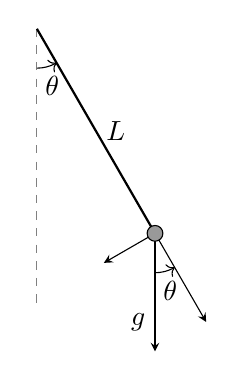
\begin{tikzpicture}
      % save length of g-vector and theta to macros
      \pgfmathsetmacro{\Gvec}{1.5}
      \pgfmathsetmacro{\myAngle}{30}
      % calculate lengths of vector components
      \pgfmathsetmacro{\Gcos}{\Gvec*cos(\myAngle)}
      \pgfmathsetmacro{\Gsin}{\Gvec*sin(\myAngle)}
      
      \coordinate (centro) at (0,0);
      \draw[dashed,gray,-] (centro) -- ++ (0,-3.5) node (mary) [black,below]{$ $};
      \draw[thick] (centro) -- ++(270+\myAngle:3) coordinate (bob) node[midway, right] {$L$};
      \pic [draw, ->, "$\theta$", angle eccentricity=1.5] {angle = mary--centro--bob};
      %\draw [blue,-stealth] (bob) -- ($(bob)!\Gcos cm!(centro)$);
      \draw [-stealth] (bob) -- ($(bob)!-\Gcos cm!(centro)$)
      coordinate (gcos)
      node[midway,above right] {};
      \draw [-stealth] (bob) -- ($(bob)!\Gsin cm!90:(centro)$)
      coordinate (gsin)
      node[midway,above left] {};
      \draw [-stealth] (bob) -- ++(0,-\Gvec)
      coordinate (g)
      node[near end,left] {$g$};
      \pic [draw, ->, "$\theta$", angle eccentricity=1.5] {angle = g--bob--gcos};
      \filldraw [fill=black!40,draw=black] (bob) circle[radius=0.1];
    \end{tikzpicture}
  \end{minipage}

  \vspace{1cm}
\end{frame}

\begin{frame}[t, c]{Two-dimensional systems}{Dissipative systems -- Attractors}
  \begin{minipage}{.48\textwidth}
    As $t \to \infty$, the dynamics of a dissipative systems settle on an \alert{\textbf{attractor}}.

    \bigskip

    For a two-dimensional system, these attractors can only be \alert{\textbf{fixed points}} or \alert{\textbf{limit cycles}}.
  \end{minipage}%
  \hfill
  \begin{minipage}{.48\textwidth}
    \centering
    \begin{tikzpicture}
      \draw[->] (-1.25*pi/2, 0) -- (1.25*pi/2, 0) node[below] {$\theta$};
      \draw[->] (0, -pi/2) -- (0, pi/2) node[left] {$\dot{\theta}$};

      \draw[gray, smooth, thick] plot file{traj1ter.txt};
      \draw[gray, smooth, thick] plot file{traj2ter.txt}; 

      \node[circle, fill=black, draw=black, inner sep=0pt, minimum size=4pt] (a) at (0, 0) {};
      \node[circle, fill=white, draw=black, inner sep=0pt, minimum size=4pt] (a) at (pi/2, 0) {};
      \node[circle, fill=white, draw=black, inner sep=0pt, minimum size=4pt] (a) at (-pi/2, 0) {};
    \end{tikzpicture}
  \end{minipage}

  \vspace{1cm}
\end{frame}

\begin{frame}[t, c]{Two-dimensional systems}{Periodic orbits in conservative systems vs. limit cycles in dissipative systems}
  \begin{minipage}{.48\textwidth}
    \centering
    \textbf{Conservative system}

    \bigskip

    \begin{tikzpicture}
      \draw[->] (-2, 0) -- (2, 0) node[below] {$\theta$};
      \draw[->] (0, -2) -- (0, 2) node[left] {$\dot{\theta}$};

      \draw[gray, smooth, thick] plot file{traj1.txt};
      \draw[gray, smooth, thick] plot file{traj2.txt};
      \draw[gray, smooth, thick] plot file{traj3.txt};
      \draw[gray, smooth, thick] plot file{traj4.txt};

      \node[circle, fill=black, draw=black, inner sep=0pt, minimum size=4pt] (a) at (0, 0) {};
      \node[circle, fill=white, draw=black, inner sep=0pt, minimum size=4pt] (a) at (1, 0) {};
      \node[circle, fill=white, draw=black, inner sep=0pt, minimum size=4pt] (a) at (-1, 0) {};
    \end{tikzpicture}
  \end{minipage}%
  \hfill
  \begin{minipage}{.48\textwidth}
    \centering
    \textbf{Dissipative system}

    \bigskip

    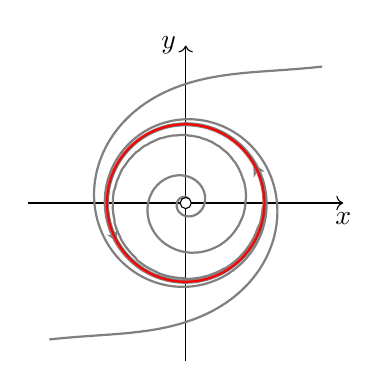
\begin{tikzpicture}
      \draw[->] (-2, 0) -- (2, 0) node[below] {$x$};
      \draw[->] (0, -2) -- (0, 2) node[left] {$y$};

      \draw[->, >=stealth, gray, domain=0:50, variable=\t, samples=1024, thick] plot ({2*sqrt(0.25*0.001 / (0.001 + exp(-0.5*\t)*(0.25-0.001))) * cos((\t+pi/4) r)}, {2*sqrt(0.25*0.001 / (0.001 + exp(-0.5*\t)*(0.25-0.001))) * sin((\t+pi/4) r)});

      \draw[->, >=stealth, gray, domain=0:50, variable=\t, samples=1024, thick] plot ({2*sqrt(0.25*1.5 / (1.5 + exp(-0.5*\t)*(0.25-1.5))) * cos((\t+pi/4) r)}, {2*sqrt(0.25*1.5 / (1.5 + exp(-0.5*\t)*(0.25-1.5))) * sin((\t+pi/4) r)});

      \draw[->, >=stealth, gray, domain=0:50, variable=\t, samples=1024, thick] plot ({2*sqrt(0.25*1.5 / (1.5 + exp(-0.5*\t)*(0.25-1.5))) * cos((\t-3*pi/4) r)}, {2*sqrt(0.25*1.5 / (1.5 + exp(-0.5*\t)*(0.25-1.5))) * sin((\t-3*pi/4) r)});

      \node[circle, fill=white, draw=black, inner sep=0pt, minimum size=4pt] (a) at (0, 0) {};

      \draw[red, thick] (0, 0) circle (1);
    \end{tikzpicture}
  \end{minipage}

  \vspace{1cm}
\end{frame}

\begin{frame}[t, c]{Two-dimensional systems}{Dissipative systems -- Volume contraction in phase space}
  \begin{minipage}{.68\textwidth}
    Thinking of the dynamics $\bm{f}(\bm{x})$ as a vector field, dissipativity can be understood as volume contraction in phase space.

    \bigskip

    Using the divergence theorem, it can easily be shown that a volume $V(t)$ of initial conditions evolves as
    %
    \[
    \dot{V} = \int_{V} \nabla \cdot \bm{f}(\bm{x})\  dV.
    \]
    %
    For a conservative system, we thus have $\nabla \cdot \bm{f}(\bm{x}) = 0 \ \forall \bm{x}$.
    For a dissipative system, we have that on average $\nabla \cdot \bm{f}(\bm{x}) < 0$.
  \end{minipage}%
  \hfill
  \begin{minipage}{.28\textwidth}
    \centering
    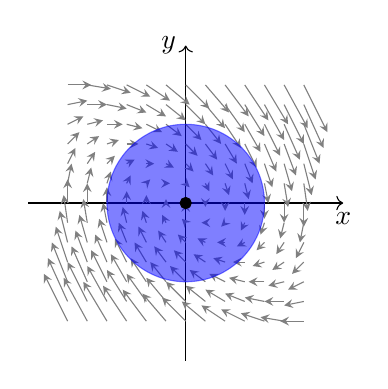
\begin{tikzpicture}
      \draw[->] (-2, 0) -- (2, 0) node[below] {$x$};
      \draw[->] (0, -2) -- (0, 2) node[left] {$y$};

      \foreach \x in {-1.5, -1.25, -1, -0.75, -0.5, -0.25, 0, 0.25, 0.5, 0.75, 1, 1.25, 1.5} {
        \foreach \y in {-1.5, -1.25, -1, -0.75, -0.5, -0.25, 0, 0.25, 0.5, 0.75, 1, 1.25, 1.5} {
          %\draw[->, >=stealth, thick]  (\x, \y) -- (\x + 0.2*\y, \y + 0.2*(- 0.5*\y - \x));
          \draw[->, gray, >=stealth]  (\x, \y) -- (\x + 0.2*\y, \y - 0.2*\y - 0.2*\x);
        }
      }

      \draw[blue, fill=blue, opacity=0.5] (0, 0) circle (1);

      \node[circle, fill=black, draw=black, inner sep=0pt, minimum size=4pt] (a) at (0, 0) {};
    \end{tikzpicture}
  \end{minipage}

  \vspace{1cm}
\end{frame}

\end{document}
